% Reproducible analytical projection: Figures/Section-CaseStudy/case_300kw.py.
\section{Illustrative Device-to-System Design Example}
\label{sec:case_study}
% Generated by case_300kw.py
\newcommand{\CaseCurrent}{205.0}
\newcommand{\CaseLegLoss}{24.97}
\newcommand{\CaseTotalLoss}{1.20}
\newcommand{\CaseEfficiency}{99.60}
\newcommand{\CaseAreaDensity}{0.37}
\newcommand{\CaseRippleWorst}{4.12}

% Generated by case_300kw.py
\newcommand{\CaseLossRows}{%
Conduction & 11.66 & 559.5 \\
Switching & 3.87 & 185.9 \\
PCB copper (load) & 7.44 & 356.9 \\
PCB copper (harmonics) & 0.99 & 47.7 \\
Capacitor ESR & 0.45 & 21.4 \\
Dead time & 0.41 & 19.8 \\
Gate drive and LDO & 0.16 & 7.5 \\
}


Figure~\ref{fig:epc2361_method} synthesizes the preceding review into an
iterative device-to-system design procedure. Electrical specifications
and the operating mission define the constraints; device voltage class,
cell count, layout, parallel count, capacitance, and switching frequency
are then evaluated together with the machine and cooling arrangement.
The verification loop revisits these choices until electrical, thermal,
and packaging requirements are met. It provides a framework for system
optimization, rather than demonstrating a global optimum.

\begin{figure*}[!t]
\centering
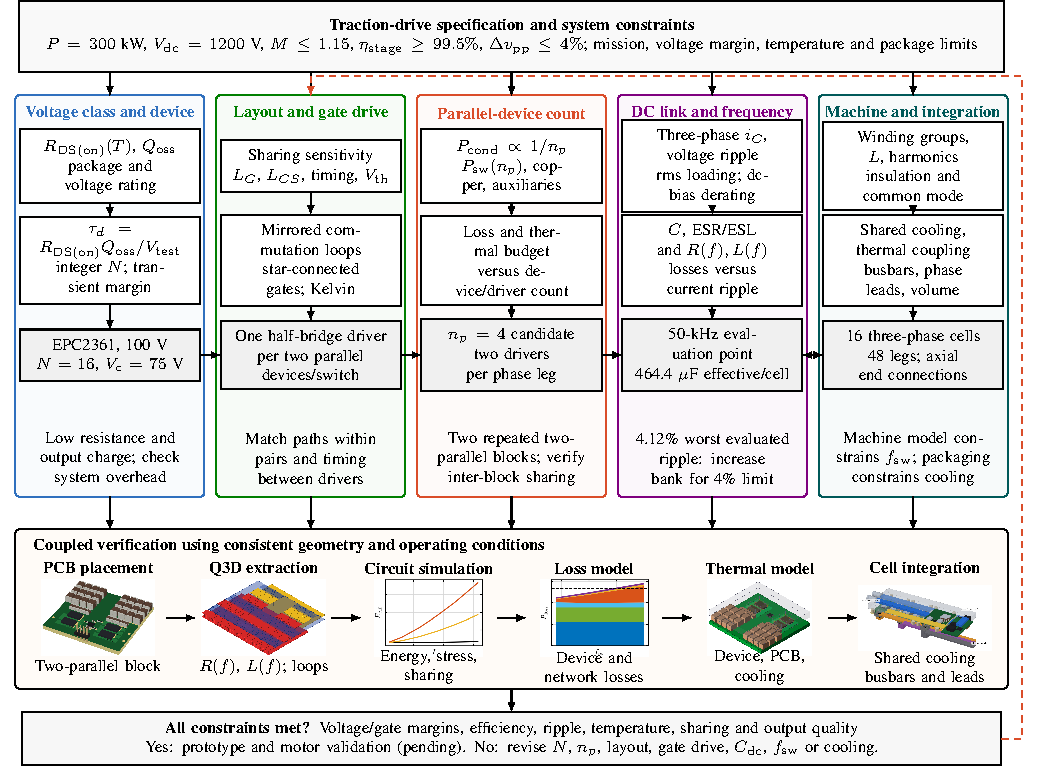
\includegraphics[width=485.600bp]{Figures/Exported/fig16.pdf}
\caption{Iterative SPB system-design procedure with coupled verification
and cell integration. Machine requirements feed back into switching-frequency,
insulation, and thermal design. Original two-parallel building-block models
support the four-parallel analytical projection; shared cooling and
interconnections require assembly-level and experimental validation.}
\label{fig:epc2361_method}
\end{figure*}

The example in Table~\ref{tab:case_300kw} uses a 300-kW, 1200-V SPB.
For balanced sinusoidal operation,
$I_{\mathrm{ph,rms}}=2\sqrt{2}P_{\mathrm{out}}/(3MV_{\mathrm{dc}}\cos\varphi)$;
$M=1.15$ and unity power factor give \CaseCurrent~A rms.
The EPC2361 is selected as an illustrative 100-V candidate: its typical
25-$^\circ$C on-resistance of 0.75~m$\Omega$, 90-nC output charge
at 50~V, and $3\times5$-mm package yield
$\tau_d=R_{\mathrm{DS(on)}}Q_{\mathrm{oss}}/V_{\mathrm{test}}=1.35$ ps
\cite{EPC2361Datasheet2026}. Sixteen cells operate at 75~V nominal;
maximum-bus operation, balancing error, and overshoot must still satisfy
\eqref{eq:semiconductor_rating}.

Four devices per switch are represented by two repeated two-parallel
blocks with matched Kelvin gate paths and two half-bridge drivers per
leg. At 50~kHz, the loss model uses on-resistance scaled to
100~$^\circ$C, sinusoidally averaged switching-energy fits, dead-time
reverse conduction, frequency-dependent PCB resistance, capacitor ESR,
and gate-drive losses. It assumes equal block currents and unchanged
local parasitics. The three-phase capacitor network accounts for dc-bias
capacitance reduction and ESR/ESL-dependent current sharing; the listed
bank requires a modest increase to meet the 4\% ripple target over the
evaluated operating points.

The projected power-stage efficiency is \CaseEfficiency\%, excluding
external isolated supplies, control electronics, inter-block busbars,
cooling auxiliaries, and machine losses. PCB-area density excludes the
cooling assembly and enclosure. Extracted inductances describe the
original block, with package and unmodeled routing inductance excluded
from the commutation value. Switching losses retain the original
terminal-energy convention, pending separation of dissipated and stored
output-capacitance energy. The 60-$^\circ$C cold-plate thermal model also
requires extension to the assembled converter and motor. Accordingly,
the design still requires verification of inter-block sharing, gate
margin, full-stack insulation, thermal coupling, and machine-current
quality, followed by experimental validation.

\begin{table}[!t]
\centering\footnotesize
\caption{300-kW SPB design inputs and preliminary repeated-block loss estimate}
\label{tab:case_300kw}
\setlength{\tabcolsep}{3pt}\renewcommand{\arraystretch}{1.04}
\begin{tabular}{@{}p{0.55\columnwidth}p{0.40\columnwidth}@{}}
\hline
Output power / dc-bus voltage & 300~kW / 1200~V\\
Cells / nominal cell voltage & 16 / 75~V\\
Devices per switch / drivers per leg & 4 / 2\\
Total devices / half-bridge drivers & 384 / 96\\
Phase current / switching frequency & \CaseCurrent~A rms / 50~kHz\\
MLCCs per phase leg & $48\times10+24\times1~\mu$F\\
Cell capacitance, nominal / effective & 1512 / 464.4~$\mu$F\\
PCB footprint per phase leg & 16.92~cm$^2$\\
Estimated efficiency / stage loss & \CaseEfficiency\% / \CaseTotalLoss~kW\\
Worst evaluated dc-link ripple & \CaseRippleWorst\% (target 4\%)\\
PCB-area power density & \CaseAreaDensity~kW/cm$^2$\\
\hline
\end{tabular}
\par\smallskip
\begin{tabular}{@{}p{0.55\columnwidth}p{0.40\columnwidth}@{}}
\hline
\multicolumn{2}{@{}l}{\textbf{Original two-parallel block: extracted layout}}\\
Board size / layer count & $30\times28.2$ mm / 4\\
Commutation loop, including capacitor ESL & 0.374 nH/local loop\\
Gate loop / Kelvin common-source inductance & 1.7 / 0.030 nH\\
\hline
\end{tabular}
\par\smallskip
\begin{tabular}{@{}lrr@{}}
\hline
\textbf{Loss component} & \textbf{Leg (W)} & \textbf{Stack (W)}\\
\hline
\CaseLossRows
\hline
Total & \CaseLegLoss & 1198.7\\
\hline
\end{tabular}
\end{table}
